\subsection{Numerical information at the summary boundary}

A new audit follows every intermediate response in the completed pilot and validation: 6,336 summaries from 3,168 hierarchical trajectories and 60 independent bases. Frozen worker reports match actual manager inputs; raw values match parsed assertions and actual root inputs throughout. The numerical-to-Boolean transformation is already present in raw model output (Fig.~\ref{fig:numeric-origin}), not introduced by parsing or serialization. Primary choice scores agree with raw answers. No rerun is indicated by this audit.

\begin{figure}[ht]\centering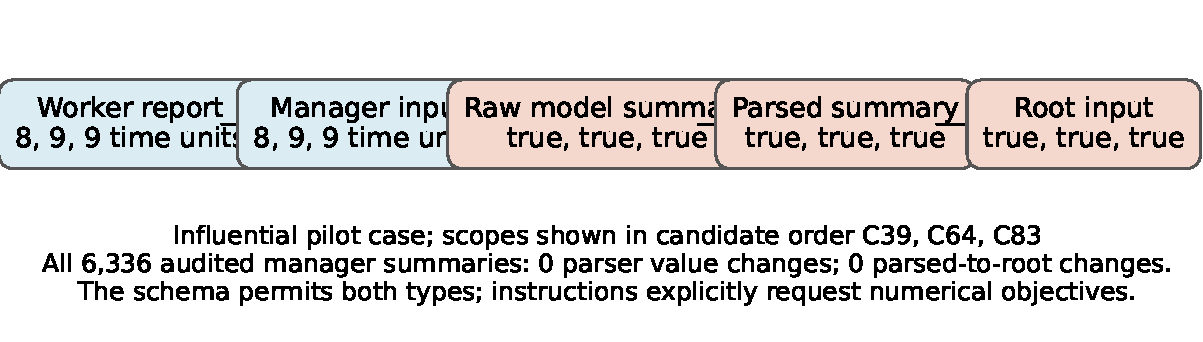
\includegraphics[width=\linewidth]{../results/numerical-pipeline-v1/figures/pipeline-origin.pdf}\caption{Observed transformation in a representative pilot trace. Scope and source references remain traceable; the numerical value is replaced in model output.}\label{fig:numeric-origin}\end{figure}

The instructions request numerical objectives, but the common assertion schema allows either Boolean or numeric values at each scope. This protocol permits the semantic error rather than enforcing scope-dependent types. Its Boolean example may be relevant, but that causal explanation is untested. These results are conditional on this interface.

\begin{table}[ht]\centering\small\caption{Boolean objective replacements in hierarchical scheduling. Denominators count full-scope candidate-objective fields, not independent samples. Pilot averages two policies; validation averages all three.}\label{tab:numeric-boolean}

\begin{tabular}{lrrr}\toprule Group & Single & Exact & Paraphrase\\\midrule

Pilot Qwen3 & 60/288 & 9/288 & 24/288\\

Validation Qwen3 & 53/648 & 64/648 & 69/648\\

Validation Phi-4 & 156/648 & 156/648 & 150/648\\

\bottomrule\end{tabular}\end{table}

The failure recurs beyond the influential pilot pair, but its reduction with repetition does not reproduce in validation (Table~\ref{tab:numeric-boolean}). Every number emitted at a known objective key in these intermediate summaries matched its source; omission and Boolean replacement were the dominant objective failures. Correctly delivered facts can still be misapplied: the complete analysis separates strict visible sufficiency from world correctness and reports both denominators. Associations conditioned on retention do not identify mediation.

Representation validity is distinct from decision support. In two of the four ill-typed baseline contexts in the fixed diagnostic, uncontested constraints already identify the sole feasible candidate. The remaining two admit multiple choices without objectives. An analysis-only supplement retains the strict invalidity labels while testing whether all admissible completions of the disputed or missing fields yield the same decision. No hidden value is restored. Missing numerical information is therefore not necessarily decision-critical; only one of the two baseline-loss bases in this small diagnostic has decision-relevant numerical uncertainty.

A separate prospective exploratory diagnostic uses six previously fixed development pairs, two with baseline objective loss and four without. Forty-eight fresh root calls cross the original upstream repetition treatment with branch-limited objective repair. Repair preserves source scope and does not add feasibility conclusions or the correct choice. It is an idealized information intervention conditional on cached summaries. Its result is pending. The existing fresh repetition confirmation does not independently confirm this interaction.
